%%%% PLEASE REPLACE ENTIRELY WITH YOUR OWN CONTENT %%%%

\chapter{Introduction}


An Introduction that clearly states the rationale of the thesis that includes:


\begin{enumerate}

  \item Statement of purpose (objectives).

  \item Requirements and specifications.

  \item Methods and procedures, citing if this work is a continuation of another project or it uses applications, algorithms, software or hardware previously developed by other authors.
  
  \item Work plan with tasks, milestones and a Gantt diagram.

  \item Description of the deviations from the initial plan and incidences that may have occurred.
\end{enumerate}
The minimum chapters that this thesis document should have are described below, nevertheless they can have different names and more chapters can be added.

\section{Work goals}
The primary objective of this project is to contribute a new methodology to the realm of molecular simulations by:

\begin{itemize} 
  \item Developing a quantum simulation program capable of efficiently modeling molecules using quantum algorithms. 
  \item Introducing innovative code that implements adaptive circuit construction and advanced optimization strategies. 
  \item Demonstrating the effectiveness of our approach by simulating selected molecular systems and comparing the results with classical computational methods. 
  \item Enhancing the integration between quantum and classical computations to optimize both electronic and nuclear degrees of freedom. 
\end{itemize}

\section{Requirements and specifications}

To achieve these objectives, the following requirements and specifications have been established:

\begin{itemize} \item \textbf{Quantum Computing Frameworks}: Utilize quantum computing libraries such as PennyLane and JAX for quantum circuit simulation and automatic differentiation. \item \textbf{Algorithm Implementation}: Implement the VQE algorithm with adaptive circuit construction, allowing the selection of the most significant excitations based on energy gradients. \item \textbf{Optimization Techniques}: Employ efficient optimizers, including gradient-based methods like gradient descent and advanced techniques like the Quantum Natural Gradient optimizer. \item \textbf{Hamiltonian Construction}: Accurately build molecular Hamiltonians for various molecular geometries and ensure compatibility with standard quantum chemistry basis sets. \item \textbf{Visualization Tools}: Develop modules for visualizing energy convergence, parameter evolution, and molecular geometries throughout the optimization process. \item \textbf{Computational Resources}: Ensure the code is optimized for performance, making effective use of computational resources and supporting parallel execution where possible. \item \textbf{Extensibility}: Design the codebase to be modular and extensible, allowing future enhancements and adaptation to other molecular systems or quantum algorithms. \end{itemize}

\section{Methods and procedures}

This project introduces innovative methods and procedures to enhance molecular simulations using quantum computing. The key innovations in our code are centered around adaptive circuit construction, advanced optimization strategies, and the seamless integration of quantum and classical computations.

\subsection*{Adaptive Circuit Construction}

Traditional VQE implementations often rely on fixed ansätze, which may not efficiently capture the complexities of all molecular systems. Our code implements an adaptive approach where the quantum circuit is dynamically constructed by selecting excitations (operators) from a predefined pool based on their contribution to lowering the system's energy. This selection is guided by computing the energy gradients with respect to each operator, ensuring that only the most impactful excitations are included in the circuit. This method enhances computational efficiency and can lead to faster convergence to the ground state energy.

\subsection*{Advanced Optimization Techniques}

Optimizing the parameters of the quantum circuit is crucial for the success of the VQE algorithm. Our implementation leverages both gradient-based and gradient-free optimization methods. We utilize optimizers like the \textit{Gradient Descent Optimizer} and explore advanced techniques such as the \textit{Quantum Natural Gradient} optimizer, which accounts for the geometry of the parameter space and can provide faster convergence. Additionally, our code extends the optimization process to include the nuclear coordinates, allowing simultaneous optimization of the electronic structure and molecular geometry.

\subsection*{Integration of Quantum and Classical Computation}

Our code exemplifies a robust integration of quantum and classical computational techniques. By employing automatic differentiation tools provided by frameworks like JAX and PennyLane, we can efficiently compute gradients of the energy with respect to both circuit parameters and nuclear coordinates. This integration facilitates the optimization process and enables the handling of complex systems that are challenging for classical methods alone.

\subsection*{Innovations in Code Implementation}

Key innovations in our code include:

\begin{itemize} \item \textbf{Dynamic Operator Selection}: A procedure to compute energy gradients for each operator in the pool and select the one with the highest impact, thus adaptively constructing the quantum circuit. \item \textbf{Hybrid Optimization Loop}: An iterative loop that updates both quantum circuit parameters and nuclear positions, enhancing the ability to find the global minimum energy configuration. \item \textbf{Efficient Gradient Computation}: Implementation of numerical methods to compute gradients with respect to nuclear coordinates, enabling geometry optimization within the VQE framework. \item \textbf{Visualization and Analysis Tools}: Development of comprehensive visualization functions to analyze the optimization process, including energy evolution plots and 3D representations of molecular geometries. \item \textbf{Modularity and Extensibility}: A modular code structure that allows for easy adaptation to different molecules, basis sets, and quantum devices, facilitating future research and development. \end{itemize}

\subsection*{Utilization of Existing Frameworks and Contribution to the Field}

While our work builds upon established quantum computing frameworks such as PennyLane and utilizes existing algorithms like the VQE, the innovations introduced in our code represent significant advancements in the field of molecular simulations. By enhancing the efficiency of quantum simulations and providing new methods for adaptive circuit construction and parameter optimization, this project contributes valuable tools and methodologies to researchers and practitioners in quantum chemistry and quantum computing.

\section{Work plan}

  \label{sec:workplan}

Normally the figures and tables are put in \verb|\figure| and \verb|\table| environments, that can float freely in the document. You can identify each float with a \verb|\label|

\begin{figure}[H]
  \centering
  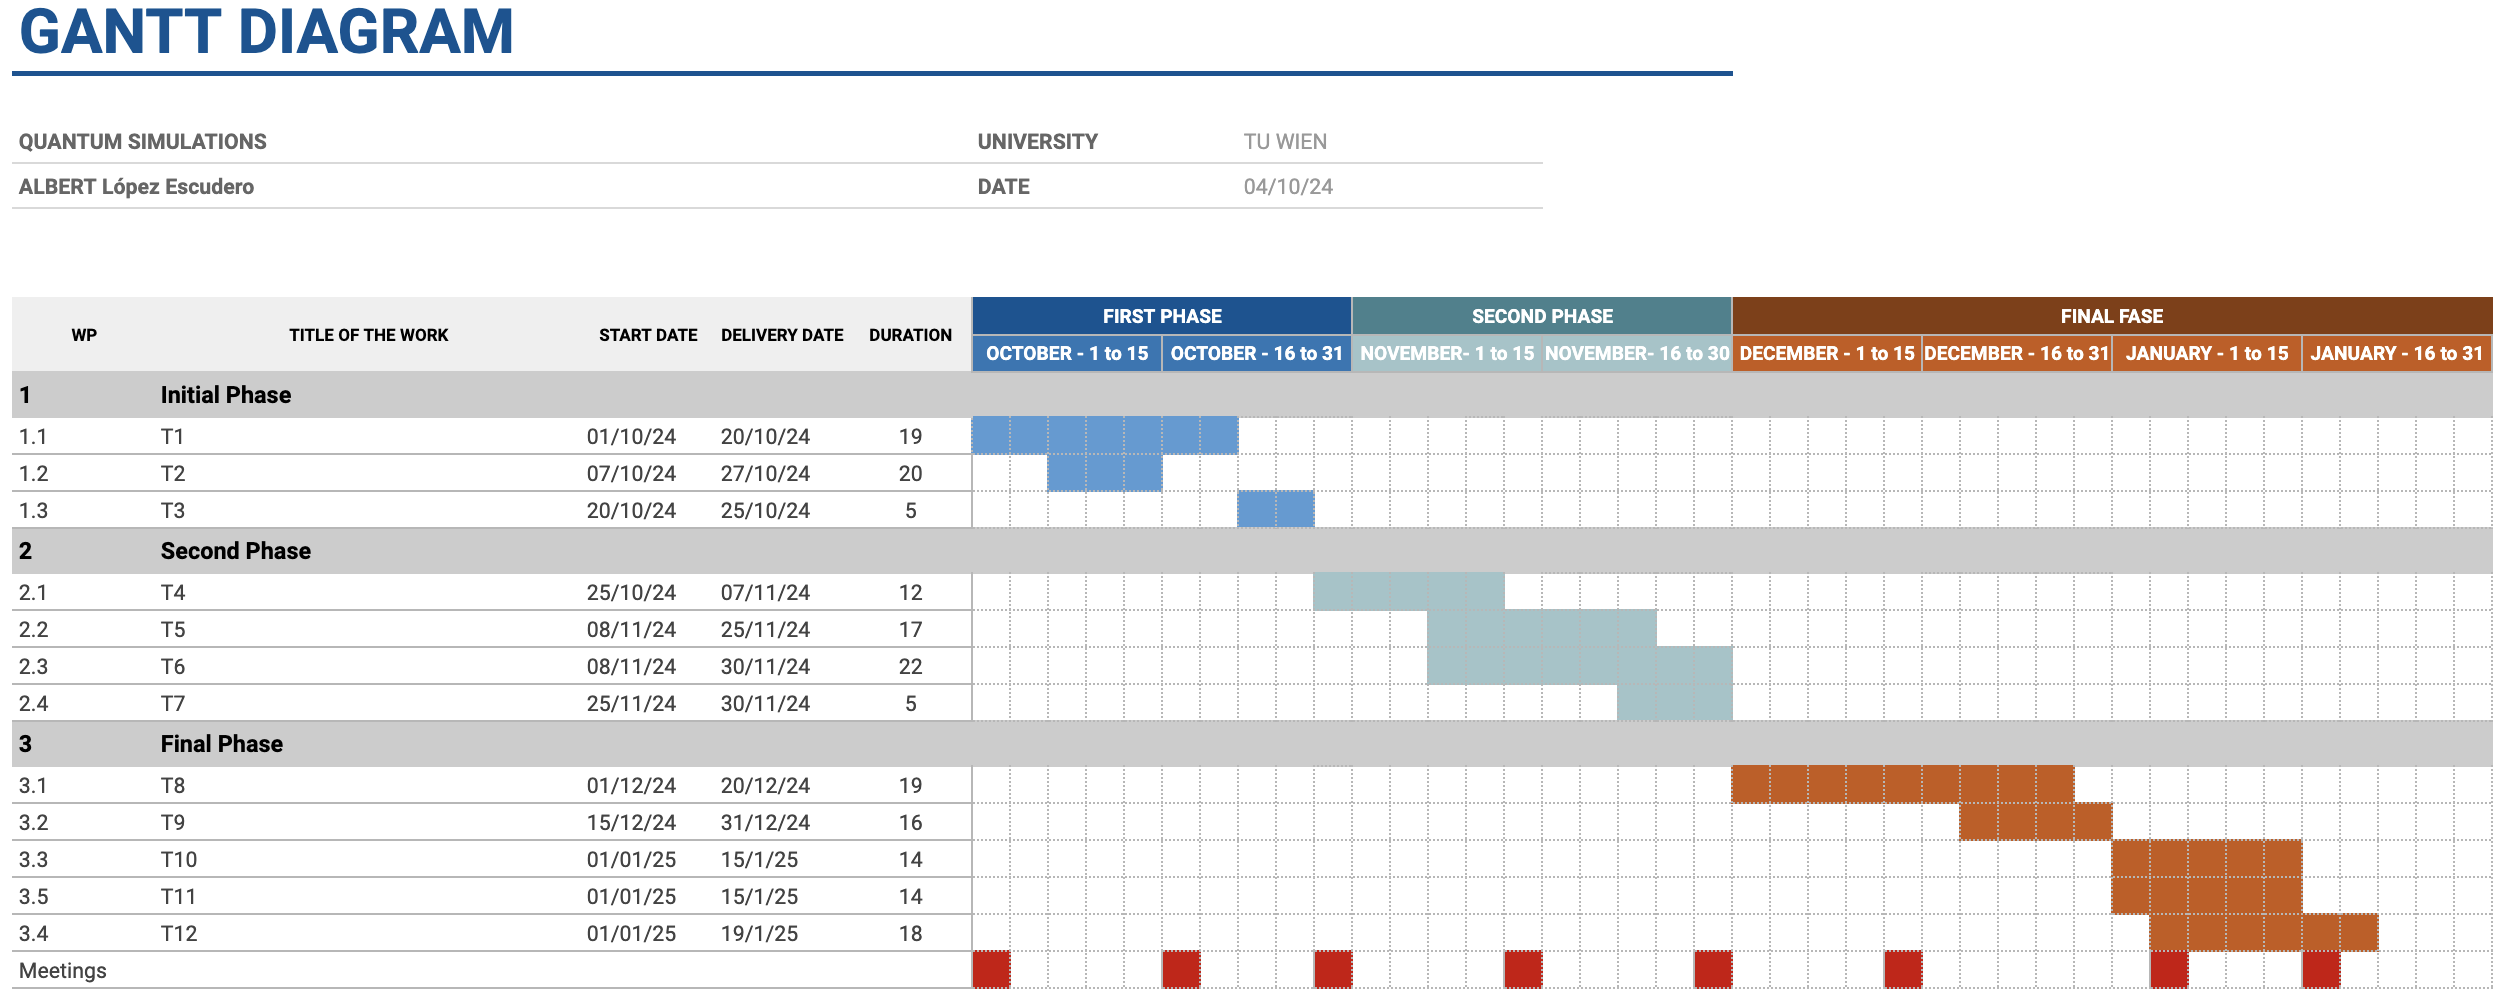
\includegraphics[width=1\textwidth]{img/Gantt_diagram.png}
  \caption{Project's Gantt diagram{\footnotesize{Gantt diagram of the project. For more information read the manual \cite{skalagantt} of Skala.}.}}
  \label{fig:gantt_diagram}
\end{figure}

